% **************************************************
% Document Class Definition
% **************************************************
\documentclass[%
    paper=A4,               % paper size --> A4 is default in Germany
    twoside=true,           % onesite or twoside printing
    openright,              % doublepage cleaning ends up right side
    parskip=half,           % spacing value / method for paragraphs
    chapterprefix=true,     % prefix for chapter marks
    11pt,                   % font size
    headings=normal,        % size of headings
    bibliography=totoc,     % include bib in toc
    listof=totoc,           % include listof entries in toc
    titlepage=on,           % own page for each title page
    captions=tableabove,    % display table captions above the float env
    chapterprefix=false,    % do not display a prefix for chapters
    appendixprefix=false,    % but display a prefix for appendix chapter
    draft=false,            % value for draft version
]{scrreprt}%


% **************************************************
% Setup YOUR thesis document in this file !
% **************************************************

\RequirePackage[					% use biblatex for bibliography
backend=biber,		% 	- use biber backend (bibtex replacement) or bibtex
style=ieee,		% 	- use alphabetic (or numeric) bib style
natbib=true,					% 	- allow natbib commands
hyperref=true,					% 	- activate hyperref support
backref=true,					% 	- activate backrefs
isbn=false,						% 	- don't show isbn tags
url=false,						% 	- don't show url tags
doi=false,						% 	- don't show doi tags
urldate=long,					% 	- display type for dates
maxnames=3,%
minnames=1,%
maxbibnames=5,%
minbibnames=3,%
maxcitenames=2,%
mincitenames=1,%,
sorting=none%
]{biblatex}
\addbibresource{bib-refs.bib}
%\addbibresource{/Users/kui07/OneDrive/Documentos/Cinvestav/Citations/Tesis.bib}


% !TEX root = my-thesis.tex


% **************************************************
% Files' Character Encoding
% **************************************************
\PassOptionsToPackage{utf8}{inputenc}
\usepackage{inputenc}


% **************************************************
% Information and Commands for Reuse
% **************************************************
\newcommand{\thesisTitle}{Análisis de los errores incurridos en la localización de fuentes de actividad neuronal al usar diversos valores nominales de conductividad cerebral}
\newcommand{\thesisName}{Óscar E. Colunga González}
\newcommand{\thesisSubject}{Documentation}
\newcommand{\thesisDate}{\today}
\newcommand{\thesisVersion}{My First Draft}

\newcommand{\thesisFirstReviewer}{Dr.\ Mauricio Carrillo Tripp}
\newcommand{\thesisFirstReviewerUniversity}{\protect{Clean Thesis Style University}}
\newcommand{\thesisFirstReviewerDepartment}{Department of Clean Thesis Style}

\newcommand{\thesisSecondReviewer}{Dr.\ Moisés Santillán Zerón}
\newcommand{\thesisSecondReviewerUniversity}{\protect{Clean Thesis Style University}}
\newcommand{\thesisSecondReviewerDepartment}{Department of Clean Thesis Style}

\newcommand{\thesisFirstSupervisor}{Dra.\ Dania Gutiérrez Ruíz}
%\newcommand{\thesisSecondSupervisor}{John Smith}

\newcommand{\thesisUniversity}{\protect{Clean Thesis Style University}}
\newcommand{\thesisUniversityDepartment}{Department of Clean Thesis Style}
\newcommand{\thesisUniversityInstitute}{Institute for Clean Thesis Dev}
\newcommand{\thesisUniversityGroup}{Clean Thesis Group (CTG)}
\newcommand{\thesisUniversityCity}{City}
\newcommand{\thesisUniversityStreetAddress}{Street address}
\newcommand{\thesisUniversityPostalCode}{Postal Code}


% **************************************************
% Debug LaTeX Information
% **************************************************
%\listfiles


% **************************************************
% Load and Configure Packages
% **************************************************
\usepackage[english]{babel} % babel system, adjust the language of the content
\PassOptionsToPackage{% setup clean thesis style
    figuresep=colon,%
    hangfigurecaption=false,%
    hangsection=true,%
    hangsubsection=true,%
    sansserif=false,%
    configurelistings=true,%
    colorize=full,%
    colortheme=bluemagenta,%
    configurebiblatex=true,%
    bibsys=bibtex,%
    bibfile=/Users/kui07/OneDrive/Documentos/Cinvestav/Citations/Tesis,%
    bibstyle=ieee,%
    bibsorting=none,%
}{cleanthesis}
\usepackage{cleanthesis}

\hypersetup{% setup the hyperref-package options
    pdftitle={\thesisTitle},    %   - title (PDF meta)
    pdfsubject={\thesisSubject},%   - subject (PDF meta)
    pdfauthor={\thesisName},    %   - author (PDF meta)
    plainpages=false,           %   -
    colorlinks=false,           %   - colorize links?
    pdfborder={0 0 0},          %   -
    breaklinks=true,            %   - allow line break inside links
    bookmarksnumbered=true,     %
    bookmarksopen=true          %
}



% **************************************************
% Document CONTENT
% **************************************************
\begin{document}

% uncomment the following command to fill up pages with
% whitespace instead of aligning the first and last lines
% of a page (see \raggedbottom vs. \flushbottom)
%\raggedbottom

% --------------------------
% rename document parts
% --------------------------
%\renewcaptionname{ngerman}{\figurename}{Abb.}
%\renewcaptionname{ngerman}{\tablename}{Tab.}
\renewcaptionname{english}{\figurename}{Fig.}
\renewcaptionname{english}{\tablename}{Tab.}
%\renewcaptionname{spanish}{\figurename}{Fig.}
%\renewcaptionname{spanish}{\tablename}{Tab.}

% --------------------------
% Front matter
% --------------------------
\pagenumbering{roman}			% roman page numbing (invisible for empty page style)
\pagestyle{empty}				% no header or footers
% !TEX root = ../my-thesis.tex
%
% ------------------------------------  --> cover title page
% \begin{titlepage}
% 	\pdfbookmark[0]{Cover}{Cover}
% 	\flushright
% 	\hfill
% 	\vfill
% 	{\LARGE\thesisTitle \par}
% 	\rule[5pt]{\textwidth}{.4pt} \par
% 	{\Large\thesisName}
% 	\vfill
% 	\textit{\large\thesisDate} \\
% 	% Versión: \thesisVersion
% \end{titlepage}


% ------------------------------------  --> main title page
\begin{titlepage}
	\pdfbookmark[0]{Titlepage}{Titlepage}
	\tgherosfont
	\centering
	
	\noindent
	%\hspace{-2cm}
	\begin{minipage}[h]{0.05\textwidth}
		\hspace{-2cm} % Move image 10 mm to the left
		
\includegraphics[width=2cm]{gfx/logospng1.png}
	\end{minipage}%
	\begin{minipage}[h]{0.95\textwidth}
		\centering
		\large 
		\textbf{CENTRO DE INVESTIGACIÓN Y DE ESTUDIOS AVANZADOS DEL INSTITUTO POLITÉCNICO NACIONAL}
	\end{minipage}


	{\large \textbf{UNIDAD MONTERREY}} \\[4mm]
	{\large \textbf{MAESTRÍA EN INGENIERÍA Y FÍSICA BIOMÉDICAS}} \\[10mm]
	
	% \large{\thesisUniversityDepartment} \\[4mm]
	%\textsf{\thesisUniversityInstitute} \\
	%\textsf{\thesisUniversityGroup} \\

	% \vfill
	% {\large \thesisSubject} \\[5mm]

	{\large \color{ctcolortitle}\textbf{\thesisTitle} \\[10mm]}
	{\large \textbf{Tesis que presenta}} \\[4mm]
	{\large \thesisName} \\[4mm]
	{\large \textbf{para obtener el grado de}} \\[4mm]
	{\large \textbf{Maestro en Ciencias}}\\[4mm]
	% \vfill
	% \begin{minipage}[t]{.27\textwidth}
	% 	\raggedleft
	% 	\textit{Sinodal}
	% \end{minipage}
	% \hspace*{15pt}
	% \begin{minipage}[t]{.65\textwidth}
	% 	{\large \thesisFirstReviewer} \\
	%   	%{\small \thesisFirstReviewerDepartment} \\[-1mm]
	% 	%{\small \thesisFirstReviewerUniversity}
	% \end{minipage} \\[5mm]
	% \begin{minipage}[t]{.27\textwidth}
	% 	\raggedleft
	% 	\textit{Sinodal}
	% \end{minipage}
	% \hspace*{15pt}
	% \begin{minipage}[t]{.65\textwidth}
	% 	{\large \thesisSecondReviewer} \\
	%   	%{\small \thesisSecondReviewerDepartment} \\[-1mm]
	% 	%{\small \thesisSecondReviewerUniversity}
	% \end{minipage} \\[10mm]
	{\large \textbf{Director de Tesis:} \thesisFirstSupervisor}
	\vfill
	\begin{flushleft}
		{\large Monterrey, Nuevo León}
		\hfill
		{\large \thesisDate}
	\end{flushleft}

\end{titlepage}


% ------------------------------------  --> lower title back for single page layout
\hfill
\vfill
{
	\small
	\textbf{\thesisName} \\
	\textit{\thesisTitle} \\
	\thesisSubject, \thesisDate \\
	Sinodales: \thesisFirstReviewer\ y \thesisSecondReviewer \\
	Directora: Dra. Dania Gutiérrez Ruiz\\[1.5em]
	\textbf{\thesisUniversity} \\
	%\textit{\thesisUniversityGroup} \\
	%\thesisUniversityInstitute \\
	\thesisUniversityDepartment \\
	\thesisUniversityStreetAddress \thesisUniversityPostalCode\\ 
	\thesisUniversityCity, México
}
		% INCLUDE: all titlepages
\cleardoublepage

\pagestyle{plain}				% display just page numbers
% !TEX root = ../my-thesis.tex
%


\pdfbookmark[0]{TODO}{TODO}
\addchap*{TODO List}

\begin{itemize}
	\item \TODO{Abstract}
	\item \TODO{Acknowledgements}
	\item \TODO{Revisar typos}
	\item \TODO{Set color to Cinvestav green} Ya agregué el color del Cinvestav, busqué el código en la página oficial y lo añadí a la plantilla. Pero no me gustó como se ve =(
	\item \TODO{Modificar las portadas y agregar el logo de Cinvestav}
	\item \TODO{Hacer versión para documento digital, actualmente el formato es para impresión}
	\item \TODO{Parte del EEG en la introducción} Parcialmente completado, falta agregar las imágenes correspondientes de las neuronas y el EEG. La parte de los generadores del EEG es la parte que tenía comentada desde que comencé a escribir, la modifiqué un poco pero no estoy seguro de que cuadre con lo demás, me gustaría su opinión al respecto. Si no le parece adecuada, puedo volver a redactarla.
	\item \TODO{Cambiar idioma a español} No tan straightforward porque hay varios comandos que se deben modificar y solo hay opciones para inglés y alemán
	\item \TODO{Modificar los comandos de la plantilla para las ecuaciones} Hecho
	\item \TODO{Remover el artículo "la" de las ecuaciones ya referenciadas para coincidir con el formato de solo escribir (x.x)}
	\item \TODO{Traducir la cita por completo}
	\item \TODO{Desarrollar la derivada parcial de la ecuación de fisher en los anexos}
	\item \TODO{Trabajo previo}
	\item \TODO{Cambiar los objetivos particulares}
	\item \TODO{Puntuación de las ecuaciones}
	\item \TODO{Agregar imágenes de los resultados preliminares a la metodología para hacer más claro el proceso} También para que cuadre el formato de la imágenes porque ya se fueron para todos lados. Igual aquí le tengo una pregunta Dra. Debería de dejar las imágenes en la parte superior de cada hoja? O hago uso de una página completa para las imágenes?
	\item \TODO{Agregar el modelo matemático de la función del dipolo}
\end{itemize}
		% INCLUDE: the abstracts (english and german)
\cleardoublepage

% !TEX root = ../my-thesis.tex
%
\pdfbookmark[0]{Abstract}{Abstract}
\addchap*{Abstract}

\blindtext

\vspace*{20mm}

{\usekomafont{chapter}Abstract (different language)}

\blindtext
		% INCLUDE: the abstracts (english and german)
\cleardoublepage
%
% !TEX root = ../my-thesis.tex
%
\pdfbookmark[0]{Acknowledgement}{Acknowledgement}
\addchap*{Acknowledgement}
\label{sec:acknowledgement}

\Blindtext[2][2]
 % INCLUDE: acknowledgement
\cleardoublepage
%
\currentpdfbookmark{\contentsname}{toc}
\setcounter{tocdepth}{2}		% define depth of toc
\tableofcontents				% display table of contents
\cleardoublepage

% --------------------------
% Body matter
% --------------------------
\pagenumbering{arabic}			% arabic page numbering
\setcounter{page}{1}			% set page counter
\pagestyle{scrheadings}			% header and footer style

%% Uncomment the following lines using the \part command
%% to add part sections
%\part{Example Part}
% !TEX root = ../my-thesis.tex
%
\chapter{Introducción}
\label{sec:intro}

%\cleanchapterquote{My own brain is to me the most unaccountable of machinery - always buzzing, humming, soaring roaring diving, and then buried in mud. And why? What's this passion for?}{Virgina Woolf}{(CEO Apple Inc.)}

\cleanchapterquote{My own brain is to me the most unaccountable of machinery - always buzzing, humming, soaring roaring diving, and then buried in mud. And why? What's this passion for?}{Virgina Woolf}

%\cleanchapterquote{Mi propio cerebro es para mi la maquinaria más inexplicable - siempre papaloteando, murmullando, }{Virgina Woolf}

\section{Electroencefalografía: Uso Clínico y Herramienta de Investigación}
\label{sec:intro:eeg}

La electroencefalografía (EEG) es una técnica no invasiva que registra la actividad eléctrica del cerebro.
Funciona mediante electrodos situados sobre el cuero cabelludo, los cuales capturan la actividad eléctrica generada por las neuronas de la corteza cerebral.
Como tal, el EEG no mide directamente la actividad neuronal, sino que registra el campo eléctrico propagado sobre el cuero cabelludo.
El EEG tiene su origen en el año 1924 cuando el médico alemán Hans Berger registró por primera vez la actividad eléctrica del cerebro humano \cite{bergerUeberElektrenkephalogrammMenschen1929}.
Desde entonces, el EEG ha sido utilizado como una herramienta clínica para el diagnóstico y monitoreo de enfermedades neurológicas como la epilepsia, trastornos del sueño, y lesiones cerebrales \cite{niedermeyerElectroencephalographyBasicPrinciples2005}.
Además, el EEG, a menudo pareado con la magnetoencefalografía (MEG), también ha sido utilizado como herramienta de investigación, particularmente en el estudio de la actividad cerebral durante estímulos sensoriales, cognitivos o motrices, que desencadenan potenciales relacionados con eventos (ERPs, del Inglés \emph{event-related potentials}) \cite{luckIntroductionEventrelatedPotential2014}.

El interés de estudiar los ERPs radica en que un conjunto de estos potenciales corresponde a la actividad eléctrica generada en la corteza cerebral en respuesta a un estímulo sensorial específico.
Estos son llamados potenciales de respuesta evocada sensorial (SEP, del Inglés \emph{sensorial-evoked potential}), y algunos ejemplos son: un sonido sostenido en cierto tono y frecuencia cambiado súbitamente en el caso de un potencial evocado auditivo (AEP, del Inglés \emph{auditory-evoked potential}), un flash de luz en un potencial evocado visual (VEP, del Inglés \emph{visual-evoked potential}), un pinchazo o estimulación eléctrica en un potencial evocado somatosensorial (SSEP, del Inglés \emph{somatosensory-evoked potential}) \cite{kreutzerEncyclopediaClinicalNeuropsychology2011}.
Estos potenciales son utilizados porque generan activaciones corticales representativas y repetibles en respuesta al estímulo, la cual es medible con el EEG, abriendo paso para la localización de las fuentes de actividad neuronal en la corteza cerebral \cite{luckIntroductionEventrelatedPotential2014}.

\section{Generadores del EEG: Corrientes Neuronales en la Corteza Cerebral}
\label{sec:intro:generators}

Con el fin de entender los conceptos con los que se trabajarán en este proyecto de tesis, ese necesario abordar los principios físico-biológicos de la generación de un EEG.

La razón por la cual existen campos electromagnéticos en la cabeza se debe a las interacciones sinápticas de las neuronas que componen el tejido cerebral.
Estas interacciones son producto de potenciales de acción generados por la depolarización de la membrana celular, lo que permite el movimiento de la descarga eléctrica a través de la red neuronal mediante las uniones de las terminales del axón de una neurona con las dendritas de otra.
Estas estructuras llamadas sinapsis pueden ser eléctricas (se comunican directamente con el paso de iones de una terminal a otra) o químicas (se comunican mediante la liberación de neurotransmisores de una terminal a otra).
Esta comunicación entre neuronas permite la transmisión de señales eléctricas del sistema nervioso central (SNC) a todo el cuerpo, o de estímulos provocados por factores externos hacía el SNC \cite{kandelPrinciplesNeuralScience2013}.

La actividad eléctrica de las neuronas puede ser medida mediante el EEG utilizando electrodos posicionados en el cuero cabelludo, pero este no puede detectar todo fenómeno eléctrico en el cerebro.
Sus limitantes son por efecto de la magnitud de los potenciales eléctricos y el tiempo en el que estos se presentan.
En el caso de los potenciales de acción, estos pueden tener una magnitud mayor (70$-$110 mV) en comparación del potencial de reposo, pero solo se producen por un pequeño lapso de tiempo (0.3 ms), además de que es raro que múltiples neuronas se activen exactamente al mismo instante, lo que imposibilita su detección por el EEG.
Mientras los potenciales post-sinápticos son menores en magnitud que los de acción (0.1$-$10 mV), el tiempo en el que estos se mantienen es mayor (10$-$20 ms), lo que permite que varias neuronas vecinas estén produciendo el mismo fenómeno eléctrico, generando así un campo eléctrico sumado que puede ser detectado por el EEG.
Cabe mencionar que las neuronas vecinas tienen que estar acomodadas en forma paralela, formando una estructura similar a una malla que potencia el fenómeno eléctrico \cite{nichollsNeuronBrain2012, Hallez2007}.

La limitante anterior es en parte producto de que el tejido del cráneo y el cuero cabelludo interfieren con la conducción del campo eléctrico generado por los potenciales de las neuronas.
Evidentemente, la conductividad eléctrica (medida en Siemens S) de los tejidos (normalmente representada por $\sigma$) que se encuentran entre el cerebro y los electrodos usados para la medición del EEG son diferentes a cero, porque permiten la detección de la actividad eléctrica en cuestión. 
La incógnita en este caso, es el valor exacto de la conductividad eléctrica de los tejidos.
Se han realizado numerosos estudios que han dado diferentes valores de dicha conductividad \cite{Gutierrez2004, McCann2019}, por lo que es de interés comparar con datos obtenidos experimentalmente, y así determinar cuáles producen resultados similares a los datos observados.

\section{Modelo Cuasi-Estático de las Leyes de Maxwell}
\label{sec:intro:physics}

El rango de frecuencias útiles de las señales electrofisiológicas captadas por el EEG y MEG es típicamente menor a 1 kHz, mientras que los fenómenos de interés se encuentran en el rango de 0.1 y 100 Hz.
Por lo tanto, la generación y propagación de estas señales puede ser descrita por la aproximación cuasi-estática de las ecuaciones de Maxwell, la cual define una aportación virtualmente nula del campo eléctrico y magnético por cambios insignificantes en el tiempo, en la propagación del campo eléctrico generado por las corrientes neuronales en la corteza cerebral \cite{Hamalainen1993, Plonsey1967}.
Bajo estas condiciones, las ecuaciones de Maxwell se simplifican de la siguiente manera:
\begin{align}
	\nabla \times B(r) & = \mu_{0} J (r) \label{eq:Maxwell} \\
	\nabla \times E(r) & = 0 \label{eq:Maxwell2}            \\
	\nabla \cdot B(r)  & = 0 \label{eq:Maxwell3}            \\
	\nabla \cdot E(r)  & = 0 \label{eq:Maxwell4}
\end{align}
donde $B(r)$ es el campo magnético, $E(r)$ es el campo eléctrico, $J(r)$ es la densidad de corriente, $\mu_{0}$ es la permeabilidad magnética, y $r = [r_x, r_y, r_z]^T$ es el punto de observación \cite{Gutierrez2008}.
En \cref{eq:Maxwell} se describe la relación entre el campo magnético y la densidad de corriente, mientras que \cref{eq:Maxwell2,eq:Maxwell3,eq:Maxwell4} describen la ausencia de fuentes magnéticas y la ausencia de carga eléctrica inducida por el cambio en el tiempo de $E$ y $B$ \cite{Hamalainen1993}.
Debido a que $E$ es irrotacional, este puede ser representado en términos del potencial eléctrico $v$ como
\begin{equation}
	E(r) = -\nabla V(r)\text{.} \label{eq:potencial}
\end{equation}

Con esta aproximación cuasi-estática, el flujo de corriente $J(r')$ en un punto $r'$ pueder ser relacionado con el campo magnético $B(r)$ en un punto $r$ mediante la ley de Biot-Savart
\begin{equation}
	B(r) = \frac{\mu_{0}}{4\pi} \int J(r') \times \frac{(r - r')}{||r - r'||^3} dV'\text{.} \label{eq:biot-savart}
\end{equation}
A su vez, la densidad de corriente total $J(r')$ puede ser dividida en dos componentes: la corriente primaria $J_{p}(r')$ que proviene de la actividad neuronal (intracelular) correspondiente al estímulo, y la corriente de volumen $J_{v}(r')$ que resulta del efecto del campo eléctrico en el tejido conductor (extracelular).
Siendo este conjunto de corrientes expresadas como
\begin{align}
	J(r') & = J^{p}(r') + J^{v}(r')\text{,} \label{eq:corriente1}               \\
	J(r') & = J^{p}(r') + \sigma(r') E(r')\text{,} \label{eq:corriente2}        \\
	J(r') & = J^{p}(r') - \sigma(r') \nabla V(r')\text{,} \label{eq:corriente3}
\end{align}
donde $\sigma(r')$ es la conductividad del tejido de la cabeza, asumiéndolo como un medio conductor isotrópico y homogéneo \cite{Baillet2001, Gutierrez2008}.

Por lo tanto, las dos ecuaciones que describen el perfil del campo eléctrico y magnético para un volumen conductor son
\begin{align}
	V_0(r) & = \frac{1}{4\pi\sigma_0} \int J^{P}(r') \cdot \frac{(r - r')}{||r - r'||^3} dr' \text{,} \label{eq:forward1} \\
	B_0(r) & = \frac{\mu_{0}}{4\pi} \int J^{P}(r') \times \frac{(r - r')}{||r - r'||^3} dr' \text{,} \label{eq:forward2}
\end{align}
siendo $V_0(r)$ el potencial eléctrico en un punto $r$ con $\sigma_{0}$ como la conductividad del medio donde se encuentra la fuente de corriente y $B_0(r)$ el campo magnético en un punto $r$ con $\mu_{0}$ como la permeabilidad magnética.

\section{Problema Directo del EEG}
\label{sec:intro:direct}

Dado que las señales de EEG se ajustan al modelo electromagnético de las ecuaciones de Maxwell en su versión cuasi-estática.
Las señales de EEG pueden ser simuladas mediante la solución del problema directo.
Este consiste en calcular el potencial eléctrico presente en el cuero cabelludo mediante el modelado de la transducción de la corriente eléctrica generada por una fuente posicionada en la corteza cerebral, en este caso siendo modelada como un dipolo eléctrico que aproxima la actividad neuronal en eventos de respuesta evocada \cite{Mosher1999, Hallez2007}.
El cálculo del potencial generado por el dipolo de corriente $\mathbf{q}$ con momento dipolar  $\mathbf{q} = [q_x,\,q_y,\,q_z]^T$ y posición $\mathbf{r}_{q} = [r_{qx},\,r_{qy},\,r_{qz}]^T$ en un medio conductor infinito con conductividad $\sigma$ se describe por: \begin{equation}
	\label{fdip}
	V(\mathbf{r},\mathbf{r}_{q},\mathbf{q})=\frac{\mathbf{q}\cdot(\mathbf{r}-\mathbf{r}_{q})}{4\pi \sigma {||\mathbf{r}-\mathbf{r}_{q}||}^{3}}\text{,}
\end{equation}
con $\mathbf{r}$ siendo la posición donde el potencial es calculado \cite{Hallez2007}.

El método de elementos de frontera (BEM, del Inglés \emph{boundary element method}) es un método numérico empleado para calcular el potencial eléctrico en la superficie de un volumen conductor. Este potencial es originado por fuentes de corriente dentro del volumen, el cual se divide en interfaces representadas mediante mallas teseladas.
Este método obtiene la proyección del campo eléctrico sobre la superficie del volumen conductor al resolver el potencial inducido por las fuentes de corriente entre las interfaces de las mallas que dividen el volumen \cite{Hallez2007}.
El BEM puede emplearse para resolver el problema directo en un modelo geométricamente realista que representa la cabeza humana como un volumen conductor \cite{Ermer2001}.

En nuestro caso, este modelo geométricamente realista sirve como el volumen conductor, mientras que las mallas representan las interfaces con distintos valores de conductividad según el tejido.
Dentro de estas mallas, las pequeñas áreas triangulares funcionan como los elementos de frontera donde se calculará el potencial inducido por el dipolo eléctrico que se encuentra en la parte más interna del modelo sobre la malla que representa la corteza cerebral, efectivamente modelando la actividad neuronal correspondiente a un ER.

El modelo matemático que describe el potencial $V(\mathbf{r})$ de cualquier punto $\mathbf{r}$ en un volumen conductor dividido por elementos de frontera se describe como una aplicación de \cref{eq:forward1} dada por
\begin{equation}
	\label{bem}
	V(r) = \frac{2\sigma_{0}}{\sigma_{k}^{-} + {\sigma_{k}^{+}}} V_{0}(r) + \frac{1}{2\pi} \sum_{j=1}^{R}\frac{\sigma_{j}^{-}-\sigma_{j}^{+}}{\sigma_{k}^{-}+\sigma_{k}^{+}} \int_{r'\varepsilon S_{j}} V(r') \frac{r'-r}{||r'-r||^3}\partial S_{j}\text{,}
\end{equation}
donde $\sigma_{0}$ corresponde al medio en el que el dipolo fuente está localizado (la malla de la corteza cerebral) y $V_{0}(\mathbf{r})$ es el potencial en $\mathbf{r}$ para un medio infinito con conductividad $\sigma_{0}$ como en la \cref{fdip};
$\sigma_{j}^{-}$ y $\sigma_{j}^{+}$ son las conductividades de los compartimentos interno y externo divididos por la interfaz $S_{j}$;
$\partial S$ es un vector orientado ortogonalmente a un elemento de superficie y $||\partial S||$ el área de ese elemento de superficie \cite{Hallez2007}.

Considerando que la solución se busca en un volumen conductor de múltiples interfaces $S_{j}$ con $\text{N}_{S_j}$ triángulos, el potencial es calculado en el centro de cada uno de estos con la \cref{bem}.
Por esta razón la integral sobre la interfaz $S_{j}$ se reescribe como una sumatoria de integrales sobre esta superficie:
\begin{equation}
	\label{bem2}
	V(r) = \frac{2\sigma_{0}}{\sigma_{r}^{-} + {\sigma_{r}^{+}}} V_{0}(r) + \frac{1}{2\pi} \sum_{k=1}^{R}\frac{\sigma_{k}^{-}-\sigma_{k}^{+}}{\sigma_{r}^{-}-\sigma_{r}^{+}} \sum_{j=1}^{N_{S_{k}}} \int_{\Delta_{S_{k,j}}} V(r') \frac{r'-r}{||r'-r||^3}\partial S_{k}\text{,}
\end{equation}
cuya integral se calcula sobre $\Delta_{S_{j},k}$, el j-ésimo triángulo en la superficie $S_{j}$, y $R$ es el número de interfaces en el volumen \cite{Hallez2007}.

Tanto en \cref{bem} como en \cref{bem2} se observa el rol que la razón entre las conductividades de los compartimentos internos y externos juega en el cálculo del potencial en el volumen conductor, ya que de esta depende el potencial inducido en cada uno de los elementos de frontera y por ende el proyectado sobre el cuero cabelludo.

Es posible reescribir \cref{bem2} como un sistema de ecuaciones lineales:
\begin{equation}
	\label{lineal}
	V = BL + V_{0},
\end{equation}
donde $V$ y $V_{0}$ son vectores que denotan el potencial buscado en cada nodo y el potencial en un medio infinito respectivamente.
$L$ corresponde a la matriz generada por las integrales, la cual depende de la geometría de las superficies y la conductividad asignada a cada una de estas \cite{Hallez2007}.

\section{Problema Inverso del EEG}
\label{sec:intro:inverse}

Mientras el problema directo se enfoca en obtener una solución para el campo eléctrico generado sobre un volumen conductor a partir de una fuente de corriente, el problema inverso consiste en identificar la posición de dichas fuentes de actividad eléctrica al modelar la amplitud de los dipolos eléctricos y seleccionando los que tengan una mayor actividad \cite{Baillet2001}.
Para su cálculo es necesario: las mediciones de EEG que en nuestro caso son las simuladas mediante el problema directo, el volumen conductor, y la matriz de ganancia con su correspondiente plantilla del sistema de EEG.

Existen muchas maneras de resolver el problema inverso neuroeléctrico. En años recientes, los métodos de filtrado espacial basados en la conformación de haces (\emph{beamforming}) han ganado popularidad.
En particular, el conformador de haces de restricciones lineales y varianza mínima (LCMV del Inglés \emph{linearly-constrained minimum variance beamfomer}) originalmente diseñado e introducido en las neurociencias en \cite{VanVeen1988, VanVeen1997}.
Este filtro espacial relaciona el campo electromagnético medido en el exterior y superficie de la cabeza con la actividad neuronal subyacente, utilizando la covarianza de las señales medidas y los modelos de actividad de las fuentes y transferencia de señal entre estas y los sensores. En nuestro caso, estos modelos corresponden a la matriz de ganancia generada con BEM.
Los coeficientes de ponderación o pesos del filtro espacial se calculan para cada ubicación en una región de interés (ROI), y su formulación es la siguiente: \linebreak Sea $x$ una señal vector de forma $M \times 1$ de datos MEG o EEG medidos con $M$ sensores, y $N$ es el número de puntos en la ROI con coordenadas $r_j$, $j = 1, ..., N$.
Entonces la fuente $y(r_j)$ en cualquier punto $r_j$ puede ser estimada como la combinación ponderada de la medición $x$ con una matriz de $M \times 3$ denominada $W(r_j)$, de forma que
\begin{equation}
	\label{beamformer}
	y(r_j) = W^{T}(r_j)x \text{.}
\end{equation}
$W(r_j)$ se conoce como el filtro espacial para una fuente en la posición $r_j$ \cite{VanVeen1997,Jaiswal2020}.
Este tipo de filtro espacial produce un beamformer o formador de haces de tipo vectorial al estimar por separado la actividad para tres orientaciones de fuente ortogonales, correspondientes a las tres columnas de la matriz.

El filtro espacial $W(r_j)$ para el conformador de haces se define como
\begin{equation}
	\label{beamformer2}
	W^{T}(r_j) = (L^{T}(r_j)C^{-1}L(r_j))^{-1}L^{T}(r_j)C^{-1} \text{.}
\end{equation}
Aquí $L(r_j)$ es la matriz de ganancia con forma $M \times 3$ que define la contribución de una fuente dipolar en la posición $r_j$ a la medición $x$, y $C$ es la matriz de covarianza calculada a partir de las mediciones de EEG o MEG.
Para realizar la localización de las fuentes utilizando LCMV, se estima la varianza resultante $\text{var}(y(r_j))$ en cada punto del espacio de la fuente \cite{VanVeen1997,Jaiswal2020}, en nuestro caso siendo la malla de la corteza cerebral, lo que resulta en
\begin{equation}
	\label{beamformer3}
	\widehat{\text{var}}(y(r_j)) = \text{traza}[L^{T}(r_j)C^{-1}L(r_j)]^{-1}.
\end{equation}

Por lo general, la señal medida está contaminada por ruido no uniformemente distribuido y por lo tanto, la varianza de la señal estimada se normaliza con la varianza del ruido proyectado $C_n$ calculada sobre parte de las mediciones en estado basal o en reposo (\emph{baseline noise}).
Esta estimación normalizada es denomida \emph{índice de actividad neural} (NAI, del Inglés \emph{neuronal activity index}) \cite{VanVeen1997} y puede expresarse como
\begin{equation}
	\label{beamformer4}
	\text{NAI}(r_j) = \frac{\text{traza}\left\{[L^{T}(r_j)C^{-1}L(r_j)]^{-1}\right\}}{\text{traza}\left\{[L^{T}(r_j)C_n^{-1}L(r_j)]^{-1}\right\}} \text{.}
\end{equation}

Al aplicar \cref{beamformer4} en todos los puntos en la ROI dentro del espacio de la fuente, las mediciones de EEG/MEG se transforman en un mapa del NAI que puede ser proyectado sobre la misma malla de la corteza cerebral del modelo geométricamente realista, efectivamente resolviendo el problema inverso.
Cabe mencionar que esta formulación es solo para un instante en el tiempo, lo que resulta en una captura de la actividad en ese momento en las mediciones de EEG/MEG, si se quiere observar el cambio de la actividad con respecto al tiempo, se tiene que calcular \cref{beamformer4} también en función del tiempo.

\section{La Razón de Conductividad Cerebro/Cráneo Como Objeto de Estudio}
\label{sec:intro:study}

La idea de estimar la razón de la conductividad cerebro/cráneo nace del uso del EEG como herramienta de localización de fuentes de actividad neuronal, las cuales son posibles de estimar con las mediciones del potencial eléctrico sobre el cuero cabelludo obtenidas de EEG en cada uno de sus electrodos, y subsecuentemente aplicando técnicas de procesamiento digital de señales en tales mediciones.
La problemática de este acercamiento es que es necesario contar con un modelo \emph{a priori} de las posibles fuentes de actividad neuronal con la finalidad de tener puntos de referencia para la proyección de las mediciones de EEG y su ajuste al modelo.
Este acercamiento a la estimación de fuentes de actividad neuronal se define como el problema directo (solución de un modelo de fuentes de actividad neuronal) y el problema inverso (solución para la localización de fuentes de actividad neuronal) del EEG \cite{Hallez2007}.
Dado que una parte del problema no puede ser resuelta sin tomar suposiciones de la solución de la otra y de los parámetros bioelectromagnéticos de los tejidos que componen la cabeza como las conductividades, este acercamiento se considera un problema abierto, en particular el problema inverso del EEG por la multitud de posibles voltajes resultantes y su inestabilidad derivada de la sensibilidad a pequeños cambios en los datos como el ruido generado por el equipo de EEG.

Cuando este procedimiento es implementado para la localización de fuentes de actividad neuronal, estas son las que se toman como variable independiente con la intención de encontrar la posición que mejor se ajusta a las mediciones, mientras que las conductividades de los tejidos se asumen como conocidas utilizando valores nominales ($0.33\text{ S/m}$ para el cerebro y $0.0042 \text{ S/m}$ para el cráneo).
Estos valores aunque son utilizados ampliamente en el área de las neurociencias \cite{Rush1968,Rush1969,Cohen1983}, han sido debatidos por múltiples estudios con acercamientos novedosos de la estimación de las conductividades obteniendo valores significativamente diferentes \cite{McCann2019}.
Hablando en términos de la razón de la conductividad cerebro/cráneo (BSCR, del Inglés \emph{brain-scalp-conductivity-ratio}) se ha documentado una diferencia hasta cuatro veces mayor (1:80 versus 1:20).
Dada la multitud de diferentes soluciones a una misma implementación del problema inverso del EEG, se puede considerar que el uso de diferentes valores de conductividad también pueden afectar al resultado y puede ser utilizado como una variable en el cálculo del problema inverso en donde el caso de estudio es la estimación de la razón de la conductividad misma. 
Teniendo en cuenta que no podemos tener dos variables independientes, tendríamos que mantener en este caso la posición de las fuentes de actividad neuronal como conocidas para la solución del problema inverso.   % INCLUDE: introduction
% !TEX root = ../my-thesis.tex
%
\chapter{Hipótesis y Objetivos}
\label{sec:obj}

\section{Hipótesis}
\label{sec:obj:hipotesis}

Existen rangos de error tolerables al definir una razón de conductividad eléctrica cerebro/cráneo en la solución del problema inverso en EEG y la tolerancia estará dictada por la frontera de Cramér-Rao.

\section{Objetivo Principal}
\label{sec:obj:main}


Implementar un método de estimación del valor de la razón entre la conductividad eléctrica cerebro/cráneo basado en el cálculo de modelos de electroencefalograma (EEG) rápidamente reconfigurables en geometrías realistas obtenidas con el método de elementos de frontera (BEM del inglés \emph{Boundary element method}).

\section{Objetivos Particulares}
\label{sec:obj:individual}

\begin{itemize}
	\item Implementar el método del cálculo de EEG rápidamente recalculable propuesto por \citeauthor{Ermer2001}\cite{Ermer2001} para el caso de una fuente de actividad cerebral conocida y valores típicos del BSCR.
	\item Calcular el costo computacional de dicha implementación para una serie de valores discretos del BSCR.
	\item Probar la aplicabilidad del método propuesto en una prueba piloto para el caso de datos reales de EEG de una respuesta sensorial evocada MODIFICAR O REMOVER.
\end{itemize}
% !TEX root = ../my-thesis.tex
%
\chapter{Trabajo Previo Relacionado}
\label{sec:related}

 Dada la naturaleza abierta del análisis de localización de fuentes de EEG utilizando la técnica de la solución del problema inverso, múltiples enfoques han sido propuestos por la comunidad científica. La gran mayoría de estas propuestas abordan la localización de fuentes de EEG como un problema de optimización, donde el objetivo es encontrar la mejor solución que se ajuste a los datos observados. Al tener como objetivo la localización de fuentes de EEG, parámetros como la conductividad de los tejidos son considerados como constantes conocidas y relegadas a un segundo plano. A diferencia de los métodos de optimización de localización de fuentes de actividad neuronal, en este trabajo se propone un enfoque basado en la variabilidad de la conductividad de los tejidos; por lo que se considera relevante revisar los antecedentes relacionados con la estimación de la conductividad de los tejidos en el contexto de la localización de fuentes de EEG. 

\section{Trabajo Relacionado 1: Review on solving the forward problem in EEG source analysis}
\label{sec:related:hallez}

Aunque el objetivo de nuestro trabajo es el análisis del error incurrido en la localización de fuentes de actividad neuronal utilizando diversos valores nominales de conductividad cerebral, este se encuentra sumamente relacionado con los métodos tradicionales de optimización de localización de dichas fuentes. Por lo que es importante revisar los antecedentes relacionados con la solución del problema directo en el análisis de fuentes de EEG.

En esta revisión, Hallez \emph{et al}. presentan diversos métodos para la solución del problema directo \cite{Hallez2007}. En particular, se mencionan los métodos de elementos de frontera (BEM), elementos finitos (FEM), y métodos de diferencia finita (FDM). Estos métodos son utilizados en conjunto con modelos geométricos que representan la cabeza humana, y que son utilizados para calcular el potencial eléctrico en la superficie del cuero cabelludo. Estos modelos pueden ser geometrías simples como esferas concéntricas, o modelos más complejos que representan la anatomía de la cabeza humana por medio de mallas tridimensionales obtenidas a partir de imágenes de resonancia magnética.

En la discusión de los métodos de solución del problema directo, se menciona que el método de elementos de frontera es de los más simples y eficientes en recursos computacionales a comparación de los otros métodos, aunque presenta algunas limitantes como la necesidad de representar la conductividad de los tejidos como isotrópica en cada capa del modelo de la cabeza (información detallada sobre las diferencias se encuentra en \cref{sec:appendix:forward_problem_comparison}). Además de que los resultados obtenidos son confiables únicamente en la superficie del cuero cabelludo, y la corteza cerebral, pero no en las regiones más profundas del cerebro. Sopesando las ventajas y desventajas de los métodos de solución del problema directo, se concluyó que en términos del enfoque de nuestro proyecto, el método de elementos de frontera es el más adecuado para el análisis de fuentes de EEG variando la conductividad de los tejidos. Esto por el hecho de que es más sencillo \TODO{es sencillo la mejor descripción en esta oración?} comparar los resultados obtenidos con diferentes valores de conductividad si estos no varían en las mallas, y por la implementación de un dipolo de corriente eléctrica como modelo de un evento de respuesta evocada que tienen como localización la corteza cerebral.

\section{Trabajo Relacionado 2: Estimating Brain Conductivities and Dipole Source Signals With EEG Arrays}
\label{sec:related:gutierrez}

Uno de los trabajos donde se aborda la localización de fuentes de EEG en el contexto de la variabilidad de la conductividad de los tejidos es el de Gutierrez \emph{et al}. En donde se propone un método para la estimación de la razón de conductividad de los tejidos que componen la cabeza humana \cite{Gutierrez2004}. La metodología propuesta en este artículo se tomó como base para el desarrollo de nuestro trabajo, con la diferencia de que este artículo, los tejidos de la cabeza humana son modelados como esferas concéntricas. Este modelo de esferas concéntricas es considerado como un antecedente al modelo geométricamente realista de la cabeza humana, y su uso era común en la literatura contemporánea a la publicación de este artículo. Cabe mencionar que los métodos de solución del problema directo utilizando geometrías realistas con BEM ya habían sido propuestos, pero su ejecución era computacionalmente costosa, por lo que el uso de esferas concéntricas era una alternativa viable para la solución del problema directo.

Gracias a la actual facilidad de acceso a equipo de cómputo con mayor capacidad de procesamiento, y al progreso en los métodos numéricos necesarios para la solución de sistemas como el BEM, es que se decidió iterar en la metodología propuesta en este artículo. Las demás diferencias entre el trabajo de Gutierrez \emph{et al}. y el nuestro se encuentran en la elección de señales de EEG, el método de solución del problema inverso, y el objetivo general de la investigación. En el artículo descrito se utilizan señales reales de EEG y MEG además de las simuladas con el fin de comparar los resultados obtenidos con ambos tipos de señales. En cuanto a la solución del problema inverso, se utilizó el método de estimación de máxima verosimilitud (MLE, del inglés \emph{maximum likelihood estimation}) y el método de estimación de máxima probabilidad a posteriori (MAP, del inglés \emph{maximum a posteriori probability}). Por último, el objetivo general de la investigación fue la estimación de la razón de conductividad de los tejidos, y la localización de fuentes de actividad neuronal en la corteza cerebral comparando con la solución del problema inverso de los datos reales contra los simulados.

En contraste, el objetivo de nuestro trabajo es la comparación de los errores incurridos en la localización de fuentes de actividad neuronal utilizando diversos valores nominales de conductividad cerebral. Por lo que se decidió utilizar señales simuladas de EEG, y BEM como método de solución del problema directo en una geometría realista compuesta por mallas tridimensionales. Además, se utilizó el método de filtrado espacial para la solución del problema inverso, y se compararon los resultados obtenidos con diferentes valores de conductividad en las mallas. Otros elementos que se comparten con el artículo en cuestión son la elección de un dipolo de corriente eléctrica como modelo de un evento de respuesta evocada, y el uso de la frontera de Crámer-Rao (CRB, del inglés \emph{Crámer-Rao bound}) como métrica de evaluación de la precisión de la localización de fuentes de actividad neuronal.

\section{Trabajo Relacionado 3: Variation in Reported Human Head Tissue Electrical Conductivity Values}
\label{sec:related:mccann}




   % INCLUDE: related work

%\part{Additional Example Part}
% !TEX root = ../my-thesis.tex
%
\chapter{Metodología}

\label{sec:methodology}
%\begin{figure}[htb]
%	
\includegraphics[width=\textwidth]{gfx/Clean-Thesis-Figure}
%	\caption{Figure example: \textit{(a)} example part one, \textit{(c)} example part two; \textit{(c)} example part three}
%	\label{fig:system:example1}
%\end{figure}

En esta sección revisamos el método propuesto para probar nuestra hipótesis junto a las consideraciones tomadas para su uso. Las divisiones principales se enfocan en: la preparación del modelo geométrico utilizado para la aproximación estructural y las propiedades bioelectromagnéticas de los tejidos incluidas las variaciones de conductividad, la solución del problema directo utilizando dipolos eléctricos que modelan puntos fijos de actividad neuronal equivalentes a respuestas evocadas (ER, del inglés \emph{Evoked response}) y un vector tridimensional de magnitud variable que representa el comportamiento de dicho dipolo, la solución del problema inverso de las señales simuladas para identificar la posición de las fuentes de actividad neuronal, y por último un análisis estadístico del estimador utilizando la frontera de Cramer-Rao para verificar su desempeño como estimador no sesgado.

\section{Método Propuesto}
\label{sec:methodology:method}

Con el objetivo de abordar el problema inverso y examinar el error asociado con el uso de distintos valores reportados de la razón de la conductividad cerebro-cráneo (BSCR, del inglés \emph{Brain-scalp-conductivity-ratio}) \cite{McCann2019} en diferentes áreas de actividad neuronal relacionadas con estímulos sensoriales; diseñamos un experimento que nos permitiría construir un estimador al implementar una solución del problema inverso con datos completamente simulados, y por ende con total control sobre las variables definidas como: la conductividad, la posición, orientación y magnitud de las fuentes de actividad neuronal, y el ruido añadido a las mediciones. El proceso del experimento es una implementación completa del problema directo e inverso del EEG con un posterior análisis estadístico, el problema directo nos permite obtener un modelo detallado de la actividad neuronal en la cabeza y simular mediciones de EEG con diferentes valores del BSCR, a su vez, el problema inverso resolverá las posiciones de las fuentes simuladas utilizando las mediciones generadas por el modelo del problema directo, y el análisis estadístico nos permitirá obtener la estimación de los valores de conductividad con base en el error incurrido en la localización de las fuentes de actividad neuronal respecto a su posición real agrupando por los distintos valores de conductividad utilizados. Basándonos en trabajo previo, decidimos implementar el filtrado espacial, en particular el propuesto en \cite{VanVeen1988} como método de la solución del problema inverso, el cual es catalogado como un método paramétrico, también conocido como ``método de dipolo de corriente equivalente'' \cite{Hallez2007}. Como su nombre lo indica, estos métodos consisten en buscar en una serie predefinida de dipolos de corriente el que mejor se ajuste en su posición y orientación a las fuentes que generaron las mediciones de EEG. 

Con el fin de realizar esta prueba de ajuste de los dipolos de corriente equivalente (solución del problema inverso) es necesario obtener la solución del problema directo. Existen varios métodos para obtener dicha solución \cite{Mosher1999}, de los cuales elegimos el método de elementos de frontera (BEM) para modelos geométricamente realistas \cite{Ermer2001}. La razón de elegir este método radica en el precedente del uso de modelos con geometrías más sencillas en estudios similares \cite{Gutierrez2004}, esto debido a que el BEM resultaba ser no viable por su elevado gasto computacional al calcular de las matrices de ganancia. En la actualidad se cuenta con mayor facilidad de acceso a equipos de cómputo con el suficiente desempeño para obtener resultados en un tiempo razonable, esto aunado al desarrollo de métodos y software mucho más eficientes \cite{open,Clerc2010} nos presenta la posibilidad de implementar el BEM para geometrías realistas como una evolución natural de los métodos utilizados anteriormente.

\begin{figure}[tb]
	\centering
	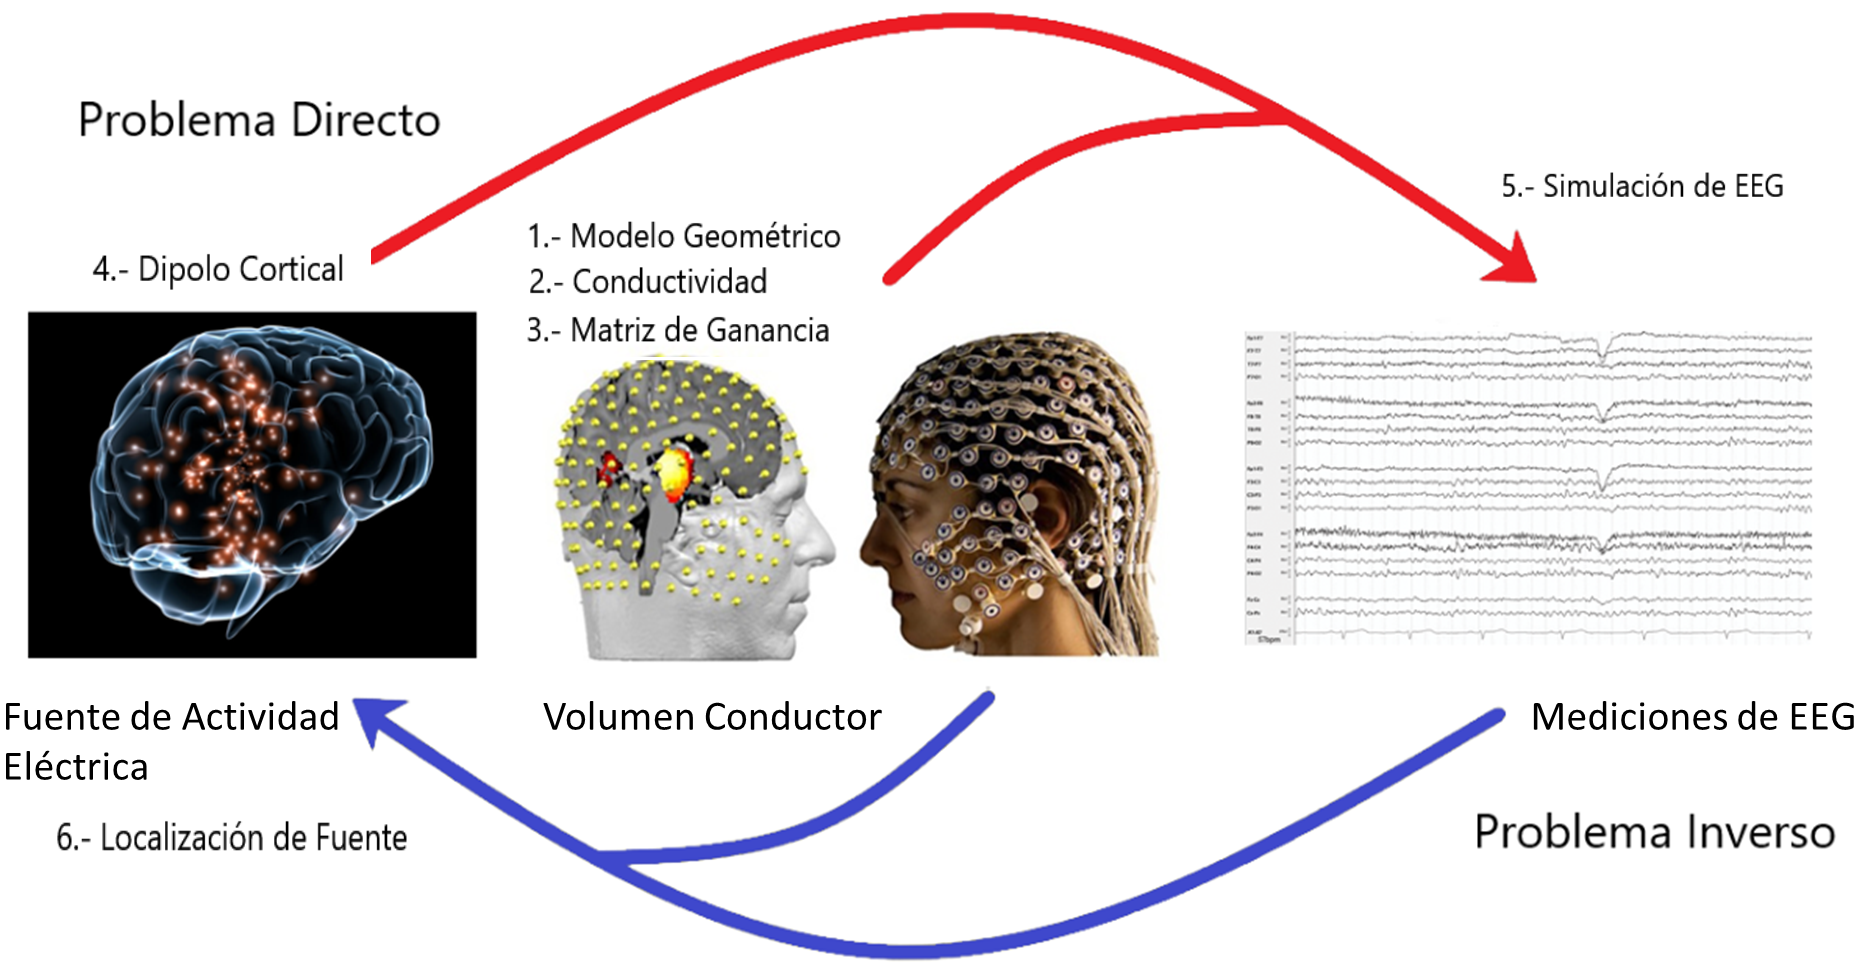
\includegraphics[width=\textwidth]{pipeline}
	\caption{Proceso del problema directo e inverso del EEG \TODO{No pude hacer más grande la imagen, la modificaré en el futuro desde la fuente}}
	\label{fig:methodology:pipeline}
\end{figure}


Una vez establecidos los métodos a utilizar en el método directo e inverso, se procedió a recopilar y formular la información necesaria para realizar los cálculos. En el caso del problema directo los datos de entrada requeridos son: el modelo geométricamente realista que representará a los tejidos de la cabeza como un volumen conductor, una serie de dipolos que modelan el fenómeno de respuesta evocada, los valores a probar de la conductividad entre los tejidos, en específico la razón cerebro/cráneo, y por último el arreglo de sensores de EEG que medirán el campo eléctrico simulado. Como resultado, se obtiene una matriz de ganancia dependiente de los valores de conductividad utilizados que dictamina como el arreglo de sensores de EEG captaría el campo eléctrico generado por las fuentes de actividad neuronal (dipolos) sobre la parte más superficial del modelo geométrico. Mientras que para el problema inverso, los datos de entrada consisten en: las mediciones de EEG simuladas a partir de la solución del problema directo, el mismo modelo geométrico con su arreglo de EEG correspondiente, las matrices de ganancia generadas en el problema directo, y las propiedades pertinentes al método de beamforming, como la matriz de covarianza de las mediciones y una matriz de covarianza del ruido. Como resultado final de este método, obtenemos un kernel de proyección de las fuentes de actividad neuronal que el beamformer pudo localizar. Lo que nos permite comparar la posición de los dipolos que fueron fijados en un principio en el problema directo contra la posición localizada por el beamformer con respecto a los diferentes valores de conductividad, y así obtener un estimador basado en los errores incurridos en la localización de estas fuentes. 


\section{Construcción del Modelo Geométricamente Realista}
\label{sec:methodology:model}

\begin{figure}[tb]
    \centering
    \begin{subfigure}{0.49\textwidth}
        \centering
        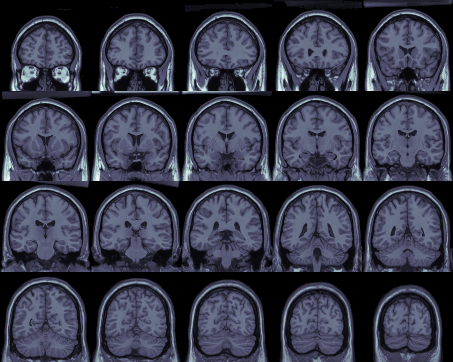
\includegraphics[width=\textwidth]{mri_coronal}
        \caption{Corte coronal}
        \label{fig:methodology:coronal}
        \vspace{0.1cm} % Add vertical space here
    \end{subfigure}
    \begin{subfigure}{0.49\textwidth}
        \centering
        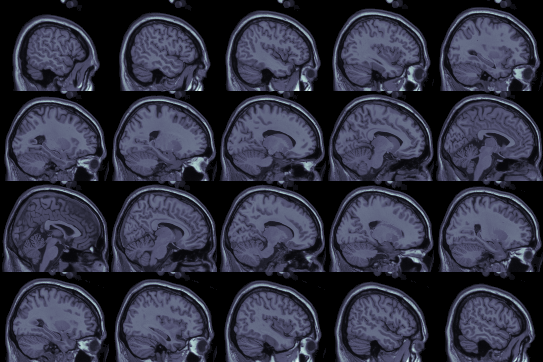
\includegraphics[width=\textwidth]{mri_sagital}
        \caption{Corte sagital}
        \label{fig:methodology:sagital}
        \vspace{0.1cm} % Add vertical space here
    \end{subfigure}
    \begin{subfigure}{0.49\textwidth}
        \centering
        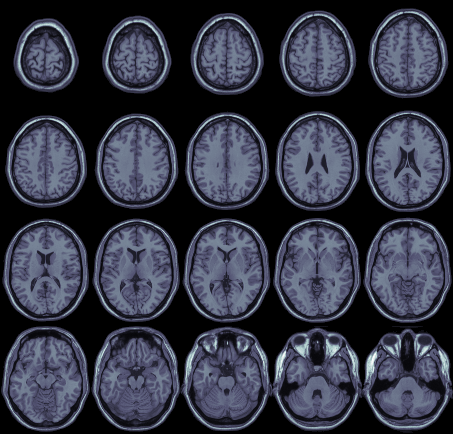
\includegraphics[width=\textwidth]{mri_axial}
        \caption{Corte axial}
        \label{fig:methodology:axial}
    \end{subfigure}
    \caption{Resonancia magnética de Colin27 \cite{Aubert-Broche2006}}
    \label{fig:methodology:mri}
\end{figure}

Entrando en detalles, la construcción del modelo geométricamente realista de los tejidos se basó en la plantilla ``Colin27 Average Brain 2008'' catalogada en \cite{Aubert-Broche2006}. Esta consiste en una versión mejorada del modelo de original de Colin que resulta del promedio de 27 imágenes de resonancia magnética ponderadas en T1, T2, y densidad protónica, provenientes de diferentes mediciones del mismo sujeto \cite{Collins1998, Holmes1998}. 

Con la información recopilada de la anatomía del sujeto se generó mediante el software libre Brainstorm\cite{brain2011} un conjunto de mallas teseladas y anidadas que representan las fases entre los diferentes tejidos de interés \emph{i.e.} cerebro, cráneo, y cuero cabelludo. Dado el alto costo computacional la resolución de las mallas es diferente dependiendo de la profundidad de las fases, siendo cerebro/cráneo y cráneo/cuero cabelludo (\cref{fig:methodology:inner,fig:methodology:outer}) las que mayor resolución tienen; 8640 triángulos y 4322 vértices, debido a que estas tienen una mayor sensibilidad al ser las más cercanas a la fuente de actividad neuronal y que representan por completo la capa de tejido óseo que servirá como volumen conductor, por estas razones es importante que ambas mallas tengan la misma resolución y no comprometan la precisión de los resultados. La fase del cuero cabelludo/aire (\cref{fig:methodology:head}) tiene una resolución menor con 6480 triángulos y 3242 vértices, esta fue definida así porque fue el límite de resolución computable con la RAM de la workstation, aún así, esta es una resolución alta comparada con el uso recomendado del software \cite{Tadel2019}. Por último se tiene una malla que representa la corteza cerebral (\cref{fig:methodology:cortex}), esta tiene una resolución de 29988 triángulos compuestos de 15002 vértices, los cuales son importantes mencionar porque la finalidad de esta malla es tener un arreglo de ``dipolos elementales'' sobre los que se proyectarán los resultados, por esta razón aunque la malla es importante para el cálculo del campo eléctrico generado por actividad neuronal no influye drásticamente en el costo computacional y puede utilizarse una resolución mayor para representar con detalle los pliegues y concavidades de la corteza cerebral. Todas las mallas en conjunto representan nuestro volumen conductor (\cref{fig:methodology:model}) sobre el que se implementarán los cálculos de BEM y la proyección del resultado del filtro espacial.

\begin{figure}[tb]
	\centering
	\begin{subfigure}{0.45\textwidth}
		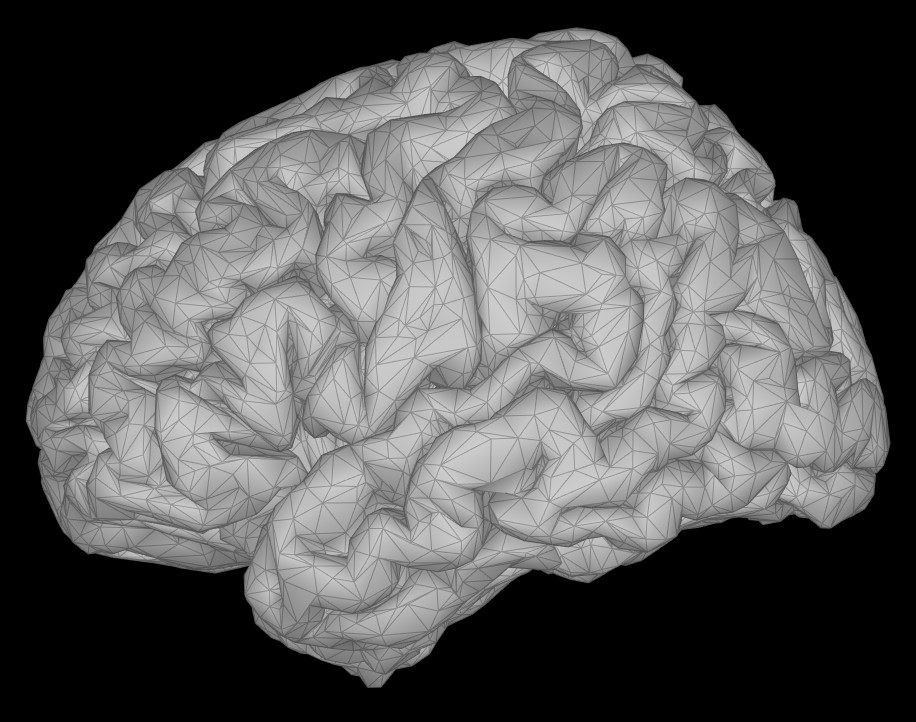
\includegraphics[width=\textwidth]{cortex}
		\caption{Corteza cerebral}
		\label{fig:methodology:cortex}
		\vspace{0.1cm}
	\end{subfigure}\hfill
	\begin{subfigure}{0.45\textwidth}
		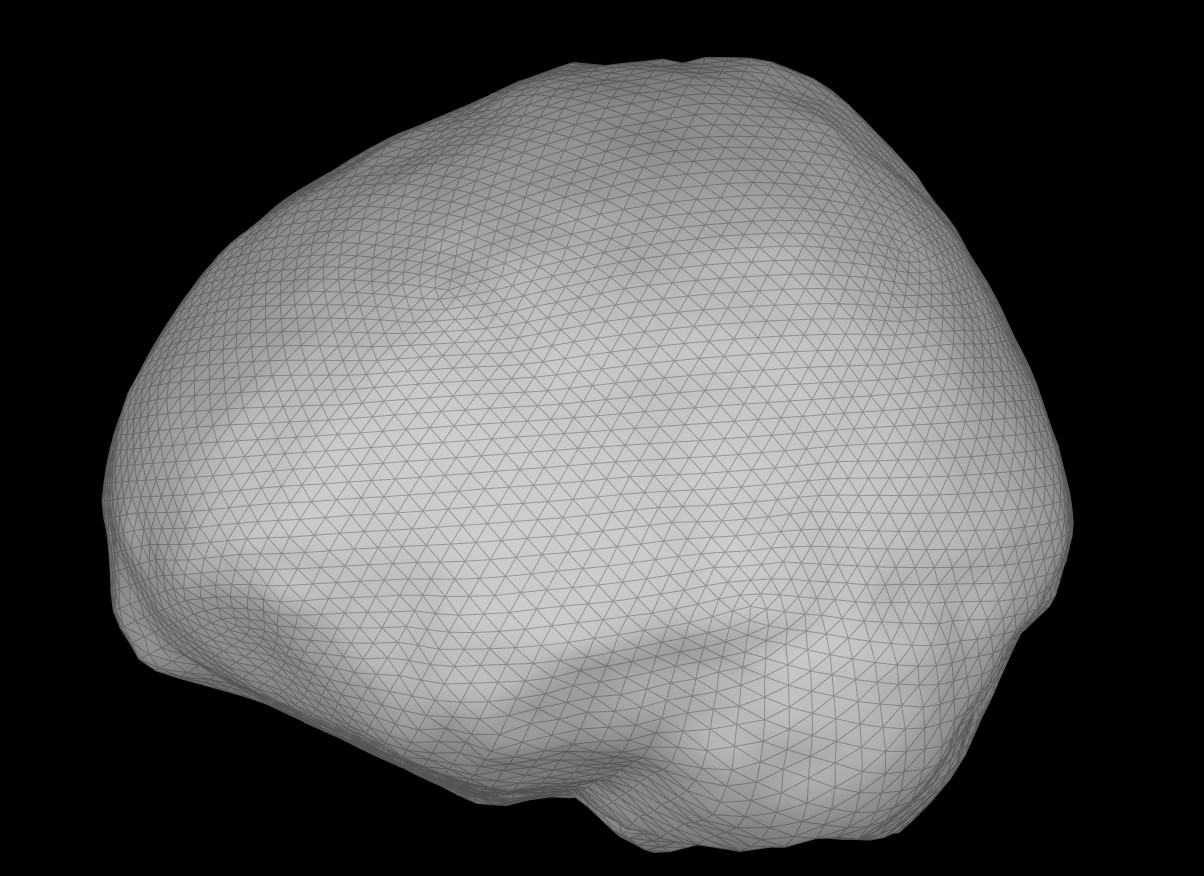
\includegraphics[width=\textwidth]{inner}
		\caption{Capa interna del cráneo}
		\label{fig:methodology:inner}
		\vspace{0.1cm}
	\end{subfigure}\\
	\begin{subfigure}{0.45\textwidth}
		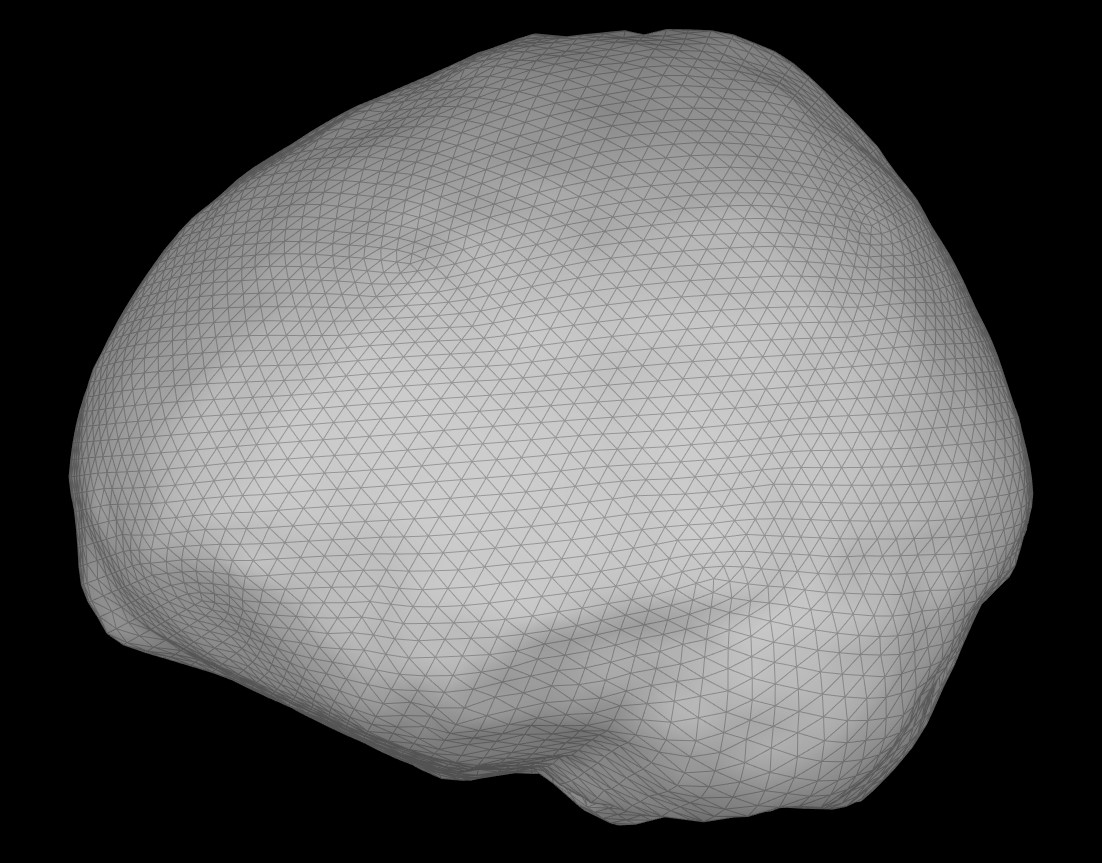
\includegraphics[width=\textwidth]{outer}
		\caption{Capa externa del cráneo}
		\label{fig:methodology:outer}
	\end{subfigure}\hfill
	\begin{subfigure}{0.45\textwidth}
		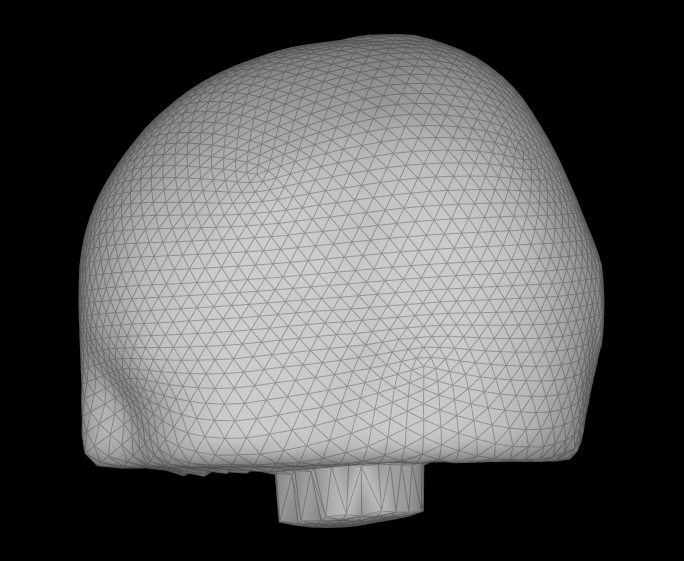
\includegraphics[width=\textwidth]{head}
		\caption{Cuero cabelludo}
		\label{fig:methodology:head}
	\end{subfigure}
	\caption{Mallas de las diferentes fases de los tejidos de la cabeza \TODO{FIX same size images and change the model}}
	\label{fig:methodology:meshes}
\end{figure}



\begin{figure}[htb]
	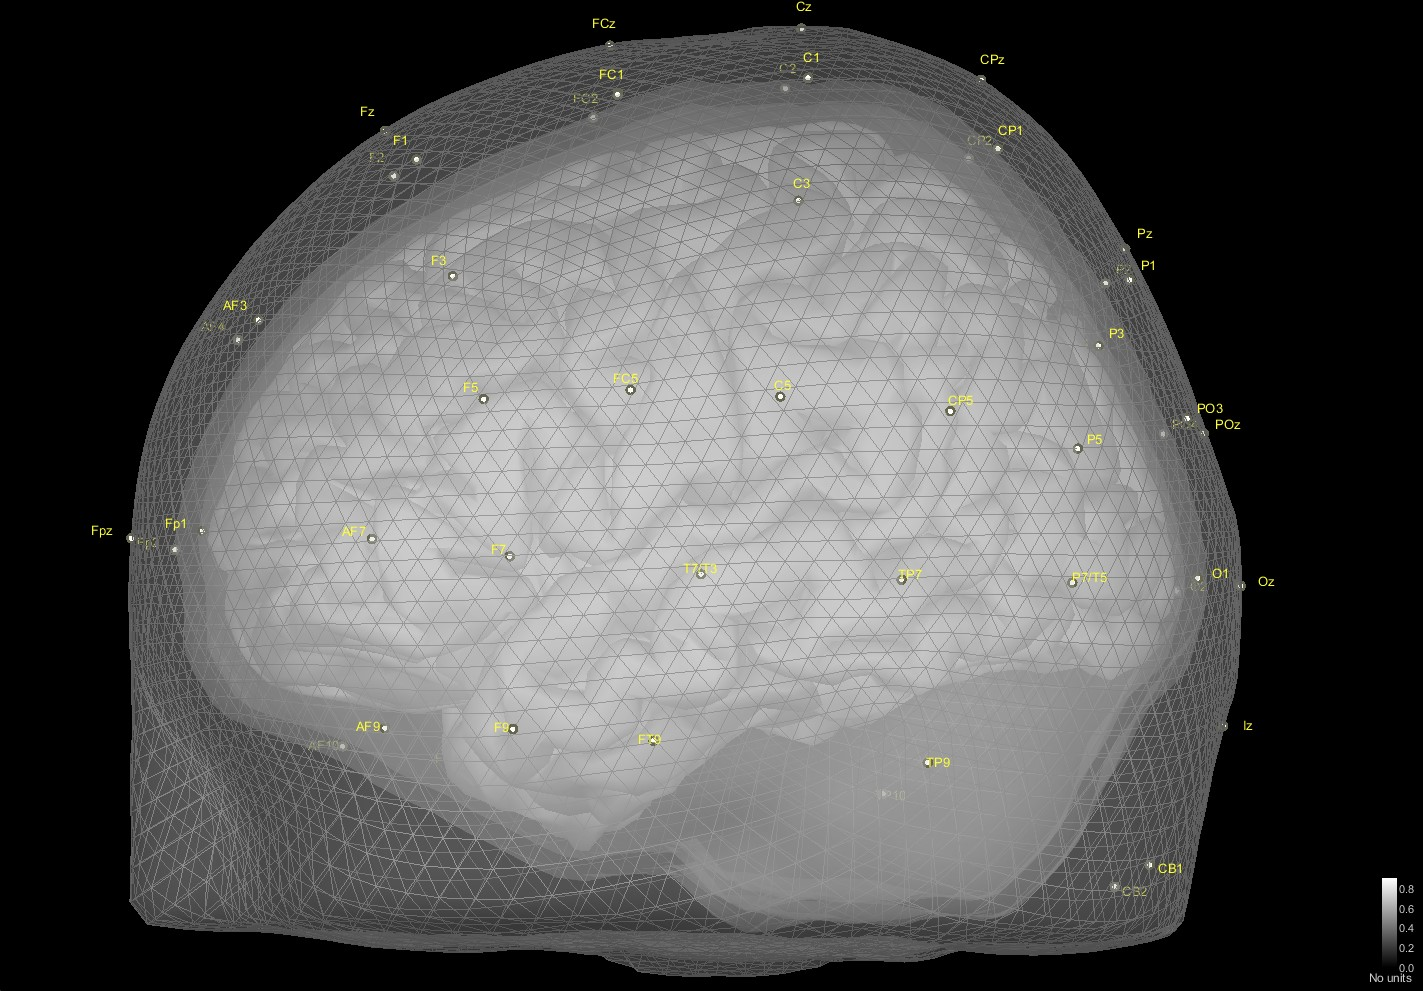
\includegraphics[width=\textwidth]{modelo}
	\caption{Modelo geométricamente realista completamente anidado}
	\label{fig:methodology:model}
\end{figure}


\section{Variación de la conductividad y cálculo de la matriz de ganancia por el método de elementos de frontera}
\label{sec:methodology:openmeeg}

Recapitulando, lo necesario para la solución del problema directo es: una fuente de corriente eléctrica y un modelo de un volumen conductor con la conductividad de los tejidos que representan. Usualmente, la finalidad de la implementación del problema directo es ubicar la posición de la fuente de corriente que representa la actividad neuronal por lo que esta ubicación es la variable independiente al momento de hacer el cálculo, mientras que la conductividad se mantiene como un valor fijo. 

En el área de neurociencias se suele mantener un valor nominal para la razón de conductividad cerebro-cráneo de 1:80 (\emph{i.e.} $0.33\text{ S/m}$ para el cerebro y $0.0042 \text{ S/m}$ para el cráneo) \cite{Rush1968,Rush1969,Cohen1983}. Sin embargo, múltiples estudios con diferentes acercamientos han publicado valores de la razón de conductividiad cerebro-cráneo que se desvían significativamente del estandár de 1:80 \cite{McCann2019}. Razón por la cual el objetivo de nuestro experimento es estimar el valor del BSCR al utilizarlo como la variable independiente mientras se toma por conocida la posición del dipolo de corriente además de mantenerse fija para todos los experimentos.

Regresando a \cref{lineal} $B$ representa la llamada \emph{matriz de ganancia} que determina la sensibilidad del arreglo de electrodos en un EEG y como estos registrarán el campo eléctrico sobre el cuero cabelludo. Para el cálculo de esta matriz de ganancia por medio de BEM se utilizó el software OpenMEEG \cite{open,open2}, donde se utilizaron como datos de entrada nuestro modelo geométricamente realista, un arreglo de EEG de 10-10 (65) \TODO{IMAGEN DEL ARREGLO}, y los valores de conductividad del cerebro, cráneo, y cuero cabelludo. Se completó el cálculo de la matriz de ganancia para 10 \TODO{TABLA DE CONDUCTIVIDADES} valores del BSCR de los cuales 2 son valores aceptados en la literatura (1:20, 1:80) y los 8 restantes se eligieron de una revisión realizada por McCann \cite{McCann2019}, el criterio para la elección de estos 8 fue el hecho que su estimación se realizó con métodos que involucraban el uso de EEG, EEG/MEG, esto con el fin de mantener relación con nuestra propia estimación y compararlos objetivamente. La matriz resultante de cada una de los valores del BSCR tiene forma de (45006 X 65), que corresponden a los 65 canales del EEG y su respuesta a los 15002 vértices de la malla de la corteza cerebral del modelo geométrico en sus tres componentes vectoriales.

\section{Dipolos de corriente e implementación de la solución del problema directo}
\label{sec:methodology:direct_solved}


\begin{figure}[tb]
	\centering
	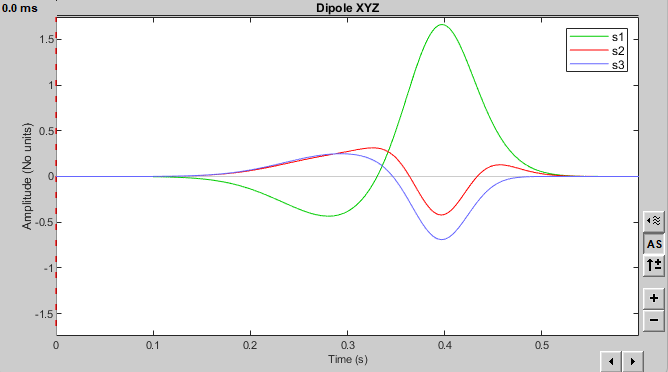
\includegraphics[width=\textwidth]{dipole-function}
	\caption{Función del dipolo eléctrico con respecto al tiempo \TODO{Añadir unidades}}
	\label{fig:methodology:dipole}
\end{figure}

La matriz de ganancia de cada BSCR con el modelo geométrico completan el volumen conductor con sus propiedades electromagnéticas, la pieza restante para el cálculo del problema directo es la fuente de actividad eléctrica que se propagará por dicho volumen conductor. Como se había discutido anteriormente se decidió usar un dipolo eléctrico de posición fija gracias a que la actividad neuronal correspondiente a un ER se puede modelar como tal, este dipolo varía su magnitud con el tiempo en un periodo de 600 ms (\cref{fig:methodology:dipole}). En cuanto a la posición, se decidió utilizar tres diferentes, cada una en distintas zonas del cerebro correspondientes a lugares de eventos de respuesta evocada, siendo estas: la corteza somatosensorial primaria (coordenadas MNI -52.2, -32.4, 55.8), corteza visual primaria (9.7, -98.6, 2.4), y corteza auditiva primaria (-65.0, -24.7, 11). Cabe mencionar que el sistema de coordenadas MNI \TODO{CITAR http://www.bic.mni.mcgill.ca/~louis/stx\_history.html} es usualmente utilizado como referencia para la comparación de diferentes sujetos, pero el software utiliza para sus cálculos el sistema CTF/MRI al que denomina \emph{Subject Coordinate System} (SCS), por lo que toda futura mención de coordenadas corresponden a dicho sistema.

Teniendo satisfechos los requisitos para la solución del problema directo este se calculó de la siguiente forma:

\begin{enumerate}
    \item Dentro del software Brainstorm, se crearon \emph{scouts} en la malla de la corteza cerebral. Estos consisten en las coordenadas SCS de las regiones de interés (ROI, del inglés \emph{region-of-interest}). Estos fueron llamados \emph{dip1} (somatosensorial), \emph{dip2} (visual), y \emph{dip3} (auditiva).
    \item Los scouts fueron utilizados como dato de entrada junto con la función del dipolo con respecto al tiempo, el volumen conductor compuesto por el modelo geométricamente realista y la matriz de ganancia de cada BSCR importadas a Brainstorm, y por último el arreglo de sensores de EEG.
    \item Como resultado, obtuvimos 100 mediciones de EEG simuladas correspondientes a cada BSCR para cada uno de los tres scouts, siendo en total 300 mediciones de EEG.
    \item Tomando en cuenta de que estamos simulando nuestros datos y estamos en control de todas las variables, se procedió a añadir ruido en la implementación del problema directo para considerar otras condiciones de experimentos con pacientes. El ruido se añadió con una relación señal/ruido (SNR, del inglés \emph{signal-to-noise-ratio}) de 0.01, 0.05, y 0.1.
    \item De esta manera, obtuvimos 3 sets de 10,000 mediciones para cada uno de los 3 dipolos, sumando a 90,000 mediciones simuladas de EEG diferentes.
\end{enumerate}

\begin{figure}[tb]
	\centering
	\begin{tikzpicture}[node distance = 3.5cm, auto]
		% Define block styles
		\tikzstyle{block} = [rectangle, draw, fill=blue!20, 
			text width=7em, text centered, rounded corners, minimum height=4em]
		\tikzstyle{line} = [draw, -{Latex}] % Use -{Latex} instead of -latex

		% Place nodes
		\node [block] (BEM) {BEM:\\Una matriz de ganancia por cada BSCR, 10 en total};
		\node [block, right of=BEM] (PD) {Problema directo:\\100 simulaciones de EEG por cada matriz de ganancia, 1,000 en total};
		\node [block, right of=PD] (SNR) {Simulación con diferente SNR:\\3 niveles de SNR, 3,000 en total};
		\node [block, right of=SNR] (Sol) {Implementación para 3 zonas diferentes de la corteza cerebral:\\9,000 en total};
		% Draw edges
		\path [line] (BEM) -- (PD);
		\path [line] (PD) -- (SNR);
		\path [line] (SNR) -- (Sol);
	\end{tikzpicture}
	\caption{Proceso del problema directo del EEG}
	\label{fig:methodology:direct_pipeline}
\end{figure}

Dado que estábamos simulando nuestros datos y teníamos control sobre todas las variables, agregamos ruido en la implementación del problema directo para simular otras condiciones de experimentación con pacientes. Este ruido se añadió con una relación señal/ruido (\emph{SNR}, del inglés \emph{signal-to-noise ratio}) de 0.01, 0.05 y 0.1. Como resultado, obtuvimos 3 conjuntos de 1,000 mediciones para cada uno de los 3 dipolos, lo que suma un total de 9,000 mediciones simuladas de EEG distintas.

\section{Implementación del Problema Inverso del EEG}
\label{sec:methodology:inverse_solved}

Dado que nuestra meta es estimar el error asociado con la resolución del problema inverso utilizando diferentes valores del BSCR en varias áreas de la corteza cerebral, implementamos la solución de la siguiente manera: Emparejamos las 100 mediciones de EEG resultantes de cada BSCR (1,000 en total) contra cada una de las 10 matrices de ganancia de los diferentes BSCR a probar, lo que resulta en 10,000 combinaciones distintas para un solo dipolo y nivel de ruido. Teniendo 3 niveles de ruido y 3 dipolos diferentes, se obtiene un total de 90,000 combinaciones distintas, y por ende; 90,000 implementaciones del problema inverso a resolver. 

\begin{figure}[tb]
	\centering
	\begin{tikzpicture}[node distance = 3.5cm, auto]
		% Define block styles
		\tikzstyle{block} = [rectangle, draw, fill=blue!20, 
			text width=7em, text centered, rounded corners, minimum height=4em]
		\tikzstyle{line} = [draw, -{Latex}] % Use -{Latex} instead of -latex

		% Place nodes
		\node [block] (1) {100 mediciones de EEG de un BSCR contra las 10 matrices de ganacia diferentes:\\1,000 en total};
		\node [block, right of=1] (2) {Expansión de cada set de mediciones de EEG por BSCR con cada matriz de ganancia:\\10,000 en total};
		\node [block, right of=2] (3) {Simulación con los 3 niveles de SNR:\\30,000 en total};
		\node [block, right of=3] (4) {Implementación para 3 zonas diferentes de la corteza cerebral:\\90,000 en total};
		% Draw edges
		\path [line] (1) -- (2);
		\path [line] (2) -- (3);
		\path [line] (3) -- (4);
	\end{tikzpicture}
	\caption{Pareamiento de mediciones de EEG con las matrices de ganancia para el problema inverso del EEG}
	\label{fig:methodology:inverse_pipeline}
\end{figure}

Al igual que en el cálculo del problema directo, se utilizó la suite Brainstorm en Matlab para el cómputo de los 90,000 conjuntos de datos; específicamente, las librerías pertinentes para el procesado de las mediciones de EEG. Estas fueron extraídas y modificadas para manejar de forma óptima el procesamiento de nuestro gran volumen de información mediante automatización y combinación de procesamientos posteriores. La razón de utilizar Brainstorm para resolver el problema inverso es que dentro de las opciones de métodos de solución incluidas se encuentra una variación del método de filtrado espacial LCMV \cite{Jaiswal2020}, este método de filtrado espacial es de interés para el laboratorio por su versatilidad y ha sido utilizado anteriormente \TODO{CITAR A EDUARDO Y DEMÁS RELACIONADO DEL LAB}.

La implementación del filtro espacial LCMV en Brainstorm obtiene mapas del pseudo-índice de actividad neuronal (PNAI, del inglés \emph{pseudo neuronal activity index}), denominado así por las modificaciones realizadas por Mosher \emph{et al.} \cite{Jaiswal2020} a la definición del índice de actividad neuronal del conformador de haces LCMV de Van Veen. En detalle, estas modificaciones consisten en el uso exclusivo de la matriz de covarianza de las mediciones de EEG para la normalización de los mapas de actividad neuronal, dejando de lado la matriz de covarianza del ruido de las mediciones de la definición original de Van Veen. 

La opción elegida de ejecución de este método de filtrado espacial sobre una medición de EEG resulta en el cálculo de un kernel de proyección del campo eléctrico detectado. Este kernel reconstruye, localiza y visualiza las fuentes de actividad neuronal en forma de mapas del PNAI sobre la serie de dipolos que componen la malla de la corteza cerebral, así como su propagación a través de las otras mallas que constituyen el modelo geométrico. Este kernel corresponde al definido por la \cref{beamformer4} con la diferencia de que la matriz de covarianza del ruido no es utilizada en el cálculo y se define como una matriz identidad. 

Tomando en cuenta que tenemos 90,000 combinaciones de mediciones de EEG y matrices de ganancia, debería de obtenerse un kernel de proyección para cada una de estas combinaciones; pero, dado que el filtro espacial tiene como datos de entrada: las mediciones de EEG, la matriz de ganancia, y la matriz de covarianza, esta última puede ser calculada a partir de las 100 mediciones de EEG de cada BSCR, obteniendo un kernel de mayor precisión que puede ser calculado para cada una de esas 100 mediciones de EEG en cualquier momento, reduciendo así el número de archivos necesarios y el espacio ocupado en el disco del equipo de cómputo. Esta fue una de las razones de realizar 100 simulaciones de EEG para cada combinación de dipolos y BSCR durante el proceso del problema directo, para mejorar la robustez del estimador y evitar sesgos durante el análisis del problema inverso. En total se obtuvieron 900 kernels de proyección, 100 por cada BSCR, para cada uno de los 3 dipolos y 3 niveles de SNR.

\section{Desarrollo del Estimador del Error de Localización de las Fuentes de Actividad Neuronal}
\label{sec:methodology:estimator}

Para la cuantización del error de localización se procedió obtener la posición de magnitud máxima de los mapas de PNAI generados por el kernel de proyección para cada uno de los 90,000 conjuntos de datos. Estos fueron separados y analizados por cada BSCR, dipolo, y nivel de SNR. La posición de magnitud máxima fue comparada con la posición real de los dipolos de corriente, y se estandarizó con la distancia media y la desviación estándar entre los vértices de los triángulos de la malla de la corteza cerebral. \TODO{Esta parte la escribí pensando en un overview del proceso, pero habiendo terminado la sección me parece redundante, me gustaría su opinión si es útil o como debería de ser redactada}

Entrando en detalle, la posición de magnitud máxima fue obtenida al implementar el kernel de proyección correspondiente a las mediciones de EEG en el instante de 397.2 ms, el cual es el mismo punto en el que se encuentra la magnitud máxima en la componente $Y$ \TODO{confirmar componente con la Dra} de la función del dipolo con respecto al tiempo, la cual corresponde al eje de la propagación del flujo eléctrico en un dipolo de corriente \TODO{abordar este punto en la introducción}. Con el fin de mejorar la precisión de la localización de la magnitud máxima, se limitó el área sobre la cual se buscó el punto máximo en el mapa de PNAI, siendo tres diferentes áreas de búsqueda, una para cada uno de los distintos dipolos: siendo estas de 29.17 cm$^2$ para el dipolo 1 correspondiendo al área de la zona somatosensorial, 51.75 cm$^2$ para el dipolo 2 correspondiente al área visual primaria, y 76.92 cm$^2$ para el dipolo 3 correspondiente al área auditiva primaria \TODO{cotejar con áreas de Brodmann, incluir imágenes y referenciarlas}. Cabe mencionar que las áreas de búsqueda se apegan a los pliegues y concavidades de la malla de la corteza cerebral, elevando el tamaño de las áreas de búsqueda y permitiendo la localización de la magnitud máxima dentro de estos pliegues.

Las posiciones de magnitud máxima de cada medición de EEG, correspondientes a sus respectivas áreas de búsqueda, fueron obtenidas en coordenadas SCS y agrupadas en sus respectivos dipolos, valor de BSCR, y niveles de SNR. Obteniendo como resultado, 900 conjuntos de 100 posiciones de magnitud máxima. Al explorar la distribución de las posiciones de magnitud máxima se observó que estas no se distribuían normalmente; como era de esperarse, la distribución de los resultados en general tenía una tendencia natural a 0, lo que generaba una distribución sesgada a la derecha, además por lo que se decidió utilizar la media del percentil P$_{95}$ como el estimador de la posición de magnitud máxima, y la distancia euclidiana entre la posición real y la posición de magnitud máxima como el estimador del error de localización \TODO{Hablar con la Dra acerca del uso de la media vs la mediana}. Una vez obtenidos los estimadores de la posición de magnitud máxima y el error de localización, se procedió a estandarizar el error de localización con respecto a la resolución de la malla de la corteza cerebral. Utilizando la distancia media y la desviación estándar entre los vértices de los triángulos de la malla de la corteza cerebral.

\section{Análisis Estadístico del Estimador}
\label{sec:methodology:statistical}

\begin{figure}[t]
	\centering
	\begin{tikzpicture}[node distance = 3.5cm, auto]
		% Define block styles
		\tikzstyle{block} = [rectangle, draw, fill=blue!20, 
			text width=7em, text centered, rounded corners, minimum height=4em]
		\tikzstyle{line} = [draw, -{Latex}] % Use -{Latex} instead of -latex

		% Place nodes
		\node [block] (1) {Ejecución del kernel de proyección para cada medición de EEG en el instante de 397.2 ms};
		\node [block, right of=1] (2) {Obtención de la posición de magnitud máxima local};
		\node [block, right of=1] (2) {Estimador de la posición de magnitud máxima y el error de localización};
		\node [block, right of=2] (3) {Estandarización del error de localización con respecto a la resolución de la malla de la corteza cerebral};
		\node [block, right of=3] (4) {Análisis estadístico del estimador con la frontera de Cramér-Rao};
		% Draw edges
		\path [line] (1) -- (2);
		\path [line] (2) -- (3);
		\path [line] (3) -- (4);
	\end{tikzpicture}
	\caption{Proceso del análisis estadístico del estimador}
	\label{fig:methodology:statistical_pipeline}
\end{figure}

Para determinar el desempeño del estimador se utilizó la frontera de Cramér-Rao (CRB, del inglés \emph{Cramér-Rao bound}), la cual proporciona un límite inferior en la varianza de los errores en la estimación de parámetros no sesgados. La CRB tiene la característica de ser universal, es decir, independiente del algoritmo utilizado para la estimación entre los no sesgados, y asintóticamente ajustado, lo que significa que para ciertas distribuciones, existen algoritmos que alcanzan el límite a medida que el número de muestras aumenta \cite{Muravchik1999,Escalona-Vargas2013}. Siendo esta última característica la de particular interés para nuestro proyecto, y una razón más para realizar las 100 simulaciones de EEG para cada combinación de dipolos, valor de BSCR, y nivel de SNR durante el proceso del problema directo.

La CRB se define como la inversa de la matriz de información de Fisher \cref{eq:crb}, la cual es el valor esperado de la segunda derivada del logaritmo de la función de verosimilitud con respecto al parámetro de interés \cref{eq:fisher}. 

\begin{equation}
	\label{eq:crb}
	\text{CRB}(\theta) = [J^{\text{EEG}}(\theta)]^{-1}
\end{equation}

\begin{equation}
    \label{eq:fisher}
    J_{ij}^{\text{EEG}}(\theta) = q^{\text{T}}\left(\pdv{k_{\infty}}{\theta_{i}}\right)^{\text{T}}\frac{\text{B}^{\text{T}}\text{B}}{\sigma^2_{\text{E}}}\left(\pdv{k_{\infty}}{\theta_{i}}\right)q
\end{equation}

\TODO{Dejar la ecuación de la matriz de información de Fisher simplificada con B como la matriz de ganancia o expandir el término?}\\
\TODO{Preguntar por formato preferido de ecuaciones, ie, coma después de la ecuación, punto y coma, punto, etc.}

Siendo la CRB el límite teórico inferior de la varianza del error del estimador no sesgado, esta se representa como una desigualdad con el valor esperado del estimador \cref{eq:crb2}.

\begin{equation}
	\label{eq:crb2}
	\text{E}\left\{(\hat{\theta} - \theta)(\hat{\theta} - \theta)^{\text{T}}\right\} \geq \text{CRB}(\theta)
\end{equation}

\TODO{Definir todas las variables de las ecuaciones}

El cálculo de la CRB se realizó con el uso de la matriz de ganancia de cada BSCR (B), el valor de la magnitud del dipolo $q$ en el instante de 397.2 ms, la derivada parcial de las posiciones de los dipolos con respecto a la posición de los sensores de EEG, y la varianza del ruido de las mediciones de EEG. Obteniendo una CRB para cada combinación de dipolos, valor de BSCR, y nivel de SNR; resultando en 90 valores de CRB.  



         % INCLUDE: system
%% !TEX root = ../my-thesis.tex
%
\chapter{Concepts: This text is here to test a very long title, to simulate the line break behavior, to show that an extremely long title also works}
\label{sec:concepts}

\cleanchapterquote{Users do not care about what is inside the box, as long as the box does what they need done.}{Jef Raskin}{about Human Computer Interfaces}

\Blindtext[2][1]

\section{Concepts Section 1}
\label{sec:concepts:sec1}

\Blindtext[2][2]

\section{Concepts Section 2 with a very very long title that illustrates how long section titles are handled in the footer}
\label{sec:concepts:sec2}

\Blindtext[3][2]

\section{Concepts Section 3}
\label{sec:concepts:sec3}

\Blindtext[4][2]

\section{Conclusion}
\label{sec:concepts:conclusion}

\Blindtext[2][1]
       % INCLUDE: concepts
%% !TEX root = ../my-thesis.tex
%
\chapter{Conclusion}
\label{sec:conclusion}

\Blindtext[2][1]

\section{System Section 1}
\label{sec:conclusion:sec1}

\Blindtext[2][2]

\section{System Section 2}
\label{sec:conclusion:sec2}

\Blindtext[3][2]

\section{Future Work}
\label{sec:conclusion:future}

\Blindtext[2][2]
     % INCLUDE: conclusion

% --------------------------
% Back matter
% --------------------------
%
{%
\setstretch{1.1}
\renewcommand{\bibfont}{\normalfont\small}
\setlength{\biblabelsep}{0pt}
\setlength{\bibitemsep}{0.5\baselineskip plus 0.5\baselineskip}
\printbibliography[nottype=online]
\newrefcontext[labelprefix={@}]
\printbibliography[heading=subbibliography,title={Webpages},type=online]
}
\cleardoublepage

\listoffigures
\cleardoublepage

\listoftables
\cleardoublepage

%\lstlistoflistings
%\cleardoublepage

%\appendix\cleardoublepage
%% !TEX root = ../my-thesis.tex
%
\chapter{Anexo}
\label{sec:appendix}

\section{Anexo: comparación	entre los métodos de solución del problema directo en el análisis de fuentes de EEG}
\label{sec:appendix:forward_problem_comparison}


\begin{table}[htb]
	\centering
	\begin{tabular}{@{}lcccc@{}}
	\toprule
											 & BEM       & FEM       & iFDM      & aFDM      \\ \midrule
	Posición de puntos computacionales       & superfice & volumen   & volumen   & volumen   \\
	Elección libre de puntos computacionales & sí        & sí        & no        & no        \\
	Sistemas matriciales                     & completos & dispersos & dispersos & dispersos \\
	Número de compartimentos                 & pequeño   & grande    & grande    & grande    \\
	Requiere teselación                      & sí        & sí        & no        & no        \\
	Anisotrópico                             & no        & sí        & no        & sí        \\ \bottomrule
	\end{tabular}
	\caption{Comparación entre los métodos de solución del problema directo en el análisis de fuentes de EEG. BEM: Boundary Element Method, FEM: Finite Element Method, iFDM: isotropic Finite Difference Method, aFDM: anisotropic Finite Difference Method.}
	\label{tab:forward_problem_comparison}
	\end{table}

\section{Anexo: comparación entre los métodos de estimación de la conductividad de los tejidos}


\begin{table}[htb]
	\begin{tabular}{@{}lll@{}}
		\toprule
		Método & Fortalezas                                                                                                                                                                       & Limitantes                                                                                                                                                    \\ \midrule
		DAC    & \begin{tabular}[c]{@{}l@{}}- No se requiere un modelo computacional\\ - Posibilidad de clasificar todo tejido\\ - Portabilidad\\ - Asequible\\ - Rápida adquisición\end{tabular} & \begin{tabular}[c]{@{}l@{}}- Invasivo\\ - Condiciones no naturales ex vivo\\ - Homogéneo\end{tabular}                                                         \\
		EIT    & \begin{tabular}[c]{@{}l@{}}- No invasivo\\ - In vivo\\ - Portable\\ - Asequible\\ - Rápida adquisición\end{tabular}                                                              & \begin{tabular}[c]{@{}l@{}}- Requiere modelo computacional\\ - Poca resolución espacial\\ - Baja relación señal/ruido\\ - Homogéneo\end{tabular}              \\
		E/MEG  & \begin{tabular}[c]{@{}l@{}}- No invasivo\\ - In vivo\\ - Portable\\ - Asequible\\ - Rápida adquisición\end{tabular}                                                              & \begin{tabular}[c]{@{}l@{}}- Requiere modelo computacional\\ - Baja resolución espacial\\ - Homogéneo\end{tabular}                                            \\
		MREIT  & \begin{tabular}[c]{@{}l@{}}- No invasivo\\ - In vivo\\ - Alta resolución espacial\\ - Anisotrópico\end{tabular}                                                                  & \begin{tabular}[c]{@{}l@{}}- Baja relación señal/ruido\\ - Señal débil en cráneo\\ - No portable\\ - Relativamente costoso\\ - Lenta adquisición\end{tabular} \\
		DTI    & \begin{tabular}[c]{@{}l@{}}- No invasivo\\ - In vivo\\ - Resolución espacial alta\\ - Anisotrópico\\ - Heterogéneo\end{tabular}                                                  & \begin{tabular}[c]{@{}l@{}}- No portable\\ - Relativamente costoso\\ - Señal débil en cráneo\\ - Lenta adquisición\end{tabular}                               \\ \bottomrule
	\end{tabular}
	\caption{Comparación entre los métodos de estimación de la conductividad de los tejidos. DAC: Dielectric Absorption Capacity, EIT: Electrical Impedance Tomography, E/MEG: Electro/Magnetoencephalography, MREIT: Magnetic Resonance Electrical Impedance Tomography, DTI: Diffusion Tensor Imaging.}
	\label{tab:conductivity_comparison}
\end{table}

       % INCLUDE: appendix

%\cleardoublepage
%% !TEX root = ../my-thesis.tex
%
\pagestyle{empty}
\hfill
\vfill
\pdfbookmark[0]{Colophon}{Colophon}
\section*{Colophon}

This thesis was typeset with \LaTeXe.
It uses the \textit{Clean Thesis} style developed by Ricardo Langner.
The design of the \textit{Clean Thesis} style is inspired by user guide documents from Apple Inc.

Download the \textit{Clean Thesis} style at \url{http://cleanthesis.der-ric.de/}.


%\cleardoublepage
%% !TEX root = ../my-thesis.tex
%
%************************************************
% Declaration
%************************************************
\pdfbookmark[0]{Declaration}{Declaration}
\addchap{Declaración de Autoría}
\label{sec:declaration}
\thispagestyle{empty}

Declaro que este trabajo es mío y que ha sido realizado únicamente con la ayuda de las referencias incluidas.


\bigskip

\noindent\textit{\thesisUniversityCity, \thesisDate}

\smallskip

\begin{flushright}
	\begin{minipage}{5cm}
		\rule{\textwidth}{1pt}
		\centering\thesisName
	\end{minipage}
\end{flushright}

%*****************************************
%*****************************************

%\clearpage

%\newpage
%
%\mbox{}

% **************************************************
% End of Document CONTENT
% **************************************************
\end{document}
